
\chapter{Sentiment Classification}
This section describes the experiments done. High level description and
execution of experiments. Detailed execution and technical details in appendix. 

%#TODO what is sentiment \\
Sentiment is described as "an attitude toward something; regard; opinion."\footnote{Sentiment - Dictionary.com: \url{http://dictionary.reference.com/browse/sentiment?s=t}}
The sentiment is the perceived positivity of the message that the user tries to
communicate. Sentiment is in many cases a personal thing, and can change from
person to person or from setting to setting.  

%#TODO why do we get it \\
Some of the motivation for acquiring the sentiment of a tweet or a sentence, is
that we can say something about a persons state of mind and from that predict
behaviour. We want to use the sentiment to make smart decisions alter. As an
example of usage it would be ideal to find a correlation between sentiment and
stock exchange, thus making us able to increase revenue based with decisions
based on the sentiment. 

%#TODO how do we use it \\
In this thesis we have two main ways of classifying tweets. Word counting and
training a classifier. Both methods require dictionaries of positive and
negative words, \ref{data:dictionaries}. In the classifier we use the dictionary
to extract features from a tweet. And with the word counting we count the
number of positive and negative words. 

\section{Manual Classification}\label{sentiment:manual_classification}
#TODO describe the process of manually classifying tweets. 

#TODO write about the obama tweet set. That most of the content is rubbish and
very difficult to label positive or negative.

\section{Word count classification}
#TODO description of method. 
Simply put we count the positive vs negative words. 

\subsection{Classification}

\paragraph{Polarity} 
\hspace{0pt}\\ 
#TODO calculating the polarity.  

The polarity of a given tweet is based on the difference in the amount of
positive verses negative words.

pos/totw - neg/totw 

\paragraph{Threshold} 
\hspace{0pt}\\ 
Threshold is the ratio of positive vs negative words that has to be present for a
tweet to be either positive of negative.

The percentage of positive words minus the percentage of negative words gives
the polarity value, or the positivity(how positive a tweet is) of a tweet. 
When actually deciding if a tweet is positive or negative we look at the
polarity value. If the polarity value is above the threshold (polarity >
threshold) the tweet is classified as positive. 

\paragraph{Examples of classification follows:} 
\hspace{0pt}\\ 
Example tweets:
\begin{itemize}
    \item t1 = “good that he was decreasing badly”
    \item t2 = “he was good for increase” 
    \item t3 = “good or bad”
\end{itemize}

Classification of t1:
\begin{itemize}
    \item pos = 1 / 6 = 0.16666
    \item neg = 2 / 6 = 0.33333
    \item polarity = pos - neg = -0.1667
    \item threshold of 0 gives negative classification
    \item threshold of 0.1 gives negative classification
    \item threshold of -0.2 gives positive classification
\end{itemize}

Classification of t2:
\begin{itemize}
    \item pos = 2 / 5 (to av fem ord) = 0.4
    \item neg = 0 / 5 = 0
    \item polarity = pos - neg = 0.4 - 0.0 = 0.4
    \item threshold = 0.4 ⇒ positive
    \item threshold = 0.5 ⇒ negative
    \item threshold = -0.1 ⇒ positive
\end{itemize}

Classification of t3:
\begin{itemize}
    \item pos = 1 / 3 = 0.3333
    \item neg = 1 / 3 = 0.3333
    \item polarity = pos - neg = 0
    \item threshold = 0 ⇒ positive
    \item threshold = 0.1 ⇒ negative
    \item threshold = -0.1 ⇒ positive
\end{itemize}

#TODO write this in full. Threshold average acc == 0.1 best. 
Further we found the best average threshold is 0.1.
From the table under we have the threshold value, and the average
classification accuracy among the 18 entries for each threshold. 

-0.1 avg: 0.631616666667
-0.2 avg: 0.616144444444
-0.3 avg: 0.60595
-0.4 avg: 0.598822222222
-0.5 avg: 0.588833333333
-0.6 avg: 0.571155555556
-0.7 avg: 0.542322222222
-0.8 avg: 0.508316666667
-0.9 avg: 0.488105555556
0.0 avg: 0.647972222222
0.1 avg: 0.651616666667
0.2 avg: 0.65115
0.3 avg: 0.643016666667
0.4 avg: 0.63055
0.5 avg: 0.612277777778
0.6 avg: 0.593483333333
0.7 avg: 0.571272222222
0.8 avg: 0.545783333333
0.9 avg: 0.530727777778

\subsection{Results}
#TODO write results from the classification of the different dictionaries. \\
Dictionaries based on their own dataset naturally scores the best. When cross
classifying we see that the bigram dictionaries score the best. With the
trigram dictionaries nearly as good as the bigram dictionaries.

#TODO write about the variations based on the datasets. \\

\paragraph{Threshold variations}
\hspace{0pt}\\
By varying the threshold we hoped to find an optimal point of which we could
separate tweets based on polarity. From the following
graphs, figure \ref{fig:threshold_graphs}, we can see no clear distinction of
one value being better than the other ones.  

In figure \ref{fig:threshold_graphs} we list the results of the experimentation
with the threshold. Table \ref{tbl:dictionary_to_threshold} lists the
dictionaries and dataset used for which graphs in figure \ref{fig:threshold_graphs}.
'kiro dataset' and 'obama dataset' columns tells which dataset that was
classified in which graph.

\begin{tabular}{ l c c }
\hspace{0pt}\\
Dictionary name and description & kiro dataset & obama dataset \\ 
Obama original, Monogram & 1 & 10 \\
LoughranMcDonald, Monogram & 2 & 11 \\
Combined Obama original and \\ LoughranMcDonald, Monogram & 3 & 12 \\
Kiro, Monogram, self compiled & 4 & 13 \\
Obama, Monogram, self compiled & 5 & 14 \\
Kiro, Bigram, self compiled & 6 & 15 \\
Obama, Bigram, self compiled & 7 & 16 \\
Kiro, Trigram, self compiled & 8 & 17 \\
Obama, Trigram, self compiled & 9 & 18 \\

\label{tbl:dictionary_to_threshold}
\end{tabular}

\begin{figure}[htb]
    \centering
    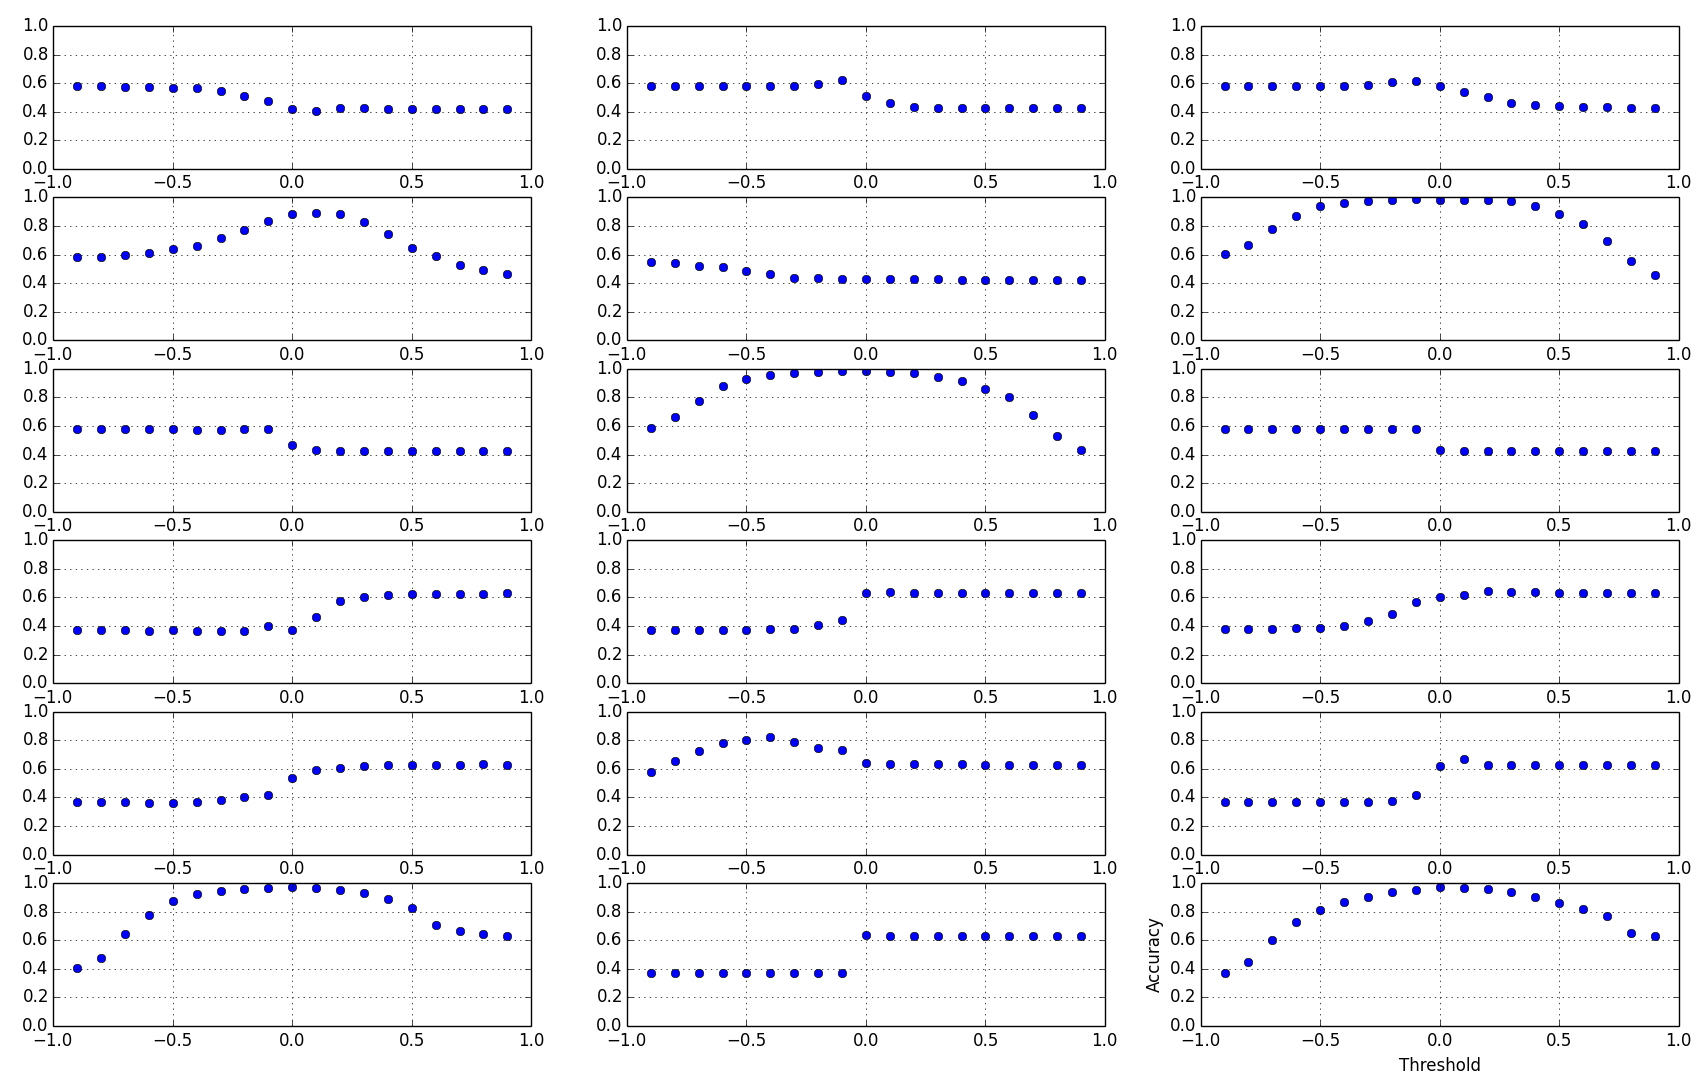
\includegraphics[width=\textwidth]{threshold_graphs.png} 
    \caption{The graphs plot the different variations of threshold. Counting is
columns first; top left is 1, top mid is 7, top right is 13.}
    \label{fig:threshold_graphs}
\end{figure}

\subsection{Drawbacks}
#TODO write about drawbacks.
\paragraph{Dictionaries}
\paragraph{Word positioning}
The dictionaries are based on the manually labeled
tweets, so we can't create bi and tri-grams based on the position of a word in a tweet.
Rather there is no way of automatically decide if a single word is positive or
negative. 

\paragraph{Threshold}
#TODO write how many tweets that end to 0 when threshold is 0.
pos-words == neg-words --> 0 but still the accuracy is quite high.

Although we can se that in line 6 we have very few cases that this happens.
From that we can can conclude that with the right choice of dictionary we don't
have the problem of the threshold value. 

0.0
null cases, 0.0 : 234 of 997
null cases, 0.0 : 543 of 997
null cases, 0.0 : 178 of 997
null cases, 0.0 : 53 of 997
null cases, 0.0 : 14 of 997
null cases, 0.0 : 7 of 997
null cases, 0.0 : 446 of 997
null cases, 0.0 : 28 of 997
null cases, 0.0 : 931 of 997
null cases, 0.0 : 335 of 1365
null cases, 0.0 : 854 of 1365
null cases, 0.0 : 345 of 1365
null cases, 0.0 : 233 of 1365
null cases, 0.0 : 37 of 1365
null cases, 0.0 : 462 of 1365
null cases, 0.0 : 52 of 1365
null cases, 0.0 : 1221 of 1365
null cases, 0.0 : 92 of 1365

\section{With Classifiers}

#TODO write about drawbacks. 

\subsection{SVM}
With both datasets.
Using the self compiled monogram dictionaries. 

Results from svm testing. which kernel works best?

\subsection{Naive Bayes}
With both datasets.
Using the self compiled monogram dictionaries. 

Results from testing with different dictionaries. 

\section{Comparison of classifiers}
#TODO highlights of the classifiers \\
#TODO common denominators. commonalities.\\
#TODO comparing the results of the classifiers. \\

\section{Comments}
#TODO improvements \\
#TODO drawbacks \\
#TODO future work \\

\section{Conclusions}
#TODO summarize the stuff we have learned shortly. \\
#TODO mention future work. \\
